\documentclass[10pt,a4paper]{article}
\usepackage[T1]{fontenc}
\usepackage[scaled]{helvet}
\usepackage{cite}
\usepackage{url}
\usepackage{graphicx}
\usepackage{float}
\usepackage{amsmath}
\usepackage{amssymb}
\usepackage{fancyhdr}
\usepackage{lastpage}
\floatstyle{boxed} 
\restylefloat{figure}
\renewcommand*\familydefault{\sfdefault}
\title{Memory, Caching and Program Execution}
\author{David Lynch}
\begin{document}
\maketitle
\begin{abstract}
We move on to introduce the concept of memory in detail, including an examination of different types of memory commonly used in computer systems. Program execution is examined in detail. Caches are ubiquitous in all kinds of computer system. This very important concept is also introduced in this section. 
\end{abstract}
\section{Memory}
Computer memory is used in various components of a computer system to store data. Fundamentally, memory is a collection of binary storage cells that is associated with transfer logic, which controls the movement of the data into and out of the CPU. Storing data into memory is accomplished by a {\bf write cycle}. Retrieving from memory is accomplished by a {\bf read cycle}. Figure \ref{mem-h} . represents how different types of memory relate to each other from a couple of different angles. Memory towards the top of the hierarchy is faster, but typically more expensive to build. This type of memory appears in small amounts in computer systems. As we move down the hierarchy capacity rises, and manufacturing is cheaper. However, memory at these layers has significantly slower and more variable access times. 
\subsection{Random Access Memory}
As the name suggests, RAM is memory is designed to be randomly accessed. The read and write cycles to and from RAM memory take a fixed amount of time, so no matter what part of memory data is written or read, the performance characteristics are the same. RAM used in various parts of the system, but most commonly as main, or system memory. RAM is also used in the I/O Subsystem, processor caches and within graphics processing units. RAM tends to be quick, with access times measured in nano-seconds. The random nature of access makes it perfect for storing instructions for programs that are ready for execution by the CPU. RAM is volatile memory and data does not persist after the power is cut. When it's random access nature is considered, flash memory is one exception to this rule. 
\newline
Serially accessed memory is orders of magnitude slower and has access times that are measured in milliseconds. The access characteristics of serial memory vary depending on what section of memory is accessed. The advantage of serially accessed memory is that it is non-volatile and data endures after the power is cut. The capacity of serial memory is usually orders of magnitude greater than RAM. Examples include DVD-ROM, Magnetic Hard Disk storage, Magnetic Tape storage. 
\subsubsection{Structure}
A word is an entity of bits that moves in and out of a memory unit as a group. 4-byte (32-bit) and 8-byte (64-bit) words are common in modern times. Each word in memory is associated with a single address. RAM is comprised of $k$ address lines which are responsible for selecting the source or target word within memory. There are $n$ data output lines which are responsible for the actual transfer of data. Lastly, there are control inputs, such as read/write indicators and chip selects, which identify which operations are currently being executed. When a RAM chip is executing a read cycle, it's read/write indicator is typically 0 (reading), it's chip select is 1 (use this chip). The RAM chip will at some point place data sourced from the location on the address lines on the data-bus using it's data lines. 
\newline\newline
Memory capacity is defined as $2^{k}$ words of $n$ bits in size. In a typical example, 16 gigabytes is the maximum addressable capacity With a 32-bit address bus. 
\subsubsection{Operations}
A write operation is used to transfer into memory a word that should be stored. 

\subsubsection{Types}
\begin{figure}
\caption{The ASCII Table\cite{LOGICDESIGN}}
\begin{center}
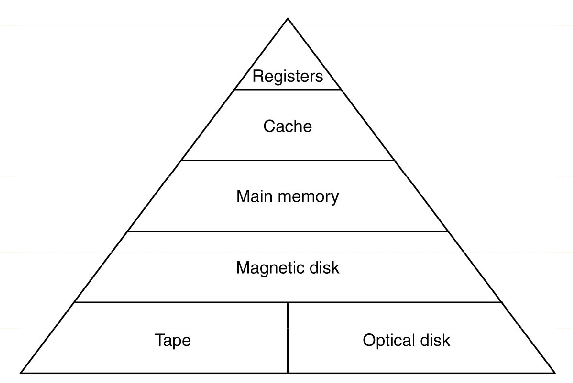
\includegraphics[scale=0.60]{../images/memory-h.png}
\label{mem-h}
\end{center}
\end{figure}
\bibliography{../biblio/techfundamentals.bib}{}
\bibliographystyle{plain}
\begin{center}
{\small \copyright  David Lynch 2012. Do not reproduce with written permission.}
\end{center}
\end{document}